\subsection{圆周角}\label{subsec:czjh2-7-5}
\begin{enhancedline}

顶点在圆上并且两边都和圆相交的角,叫做\zhongdian{圆周角}。
图 \ref{fig:czjh2-7-20} 各圆中的 $\angle BAC$ 都是圆周角。

\begin{dingli}[定理]
    一条弧所对的圆周角等于它所对的圆心角的一半。
\end{dingli}

已知: $\yuan\,O$ 中, $\yuanhu{BC}$ 所对的圆周角是 $\angle BAC$,圆心角是 $\angle BOC$ (图 \ref{fig:czjh2-7-20})。

\begin{figure}[htbp]
    \centering
    \begin{minipage}[b]{4cm}
        \centering
        \begin{tikzpicture}
    \tkzDefPoints{0/0/O}
    \tkzDefPoint(55:1.5){A}
    \tkzDefPoint(235:1.5){B}
    \tkzDefPoint(330:1.5){C}

    \tkzDrawCircle[thick](O,A)
    \tkzDrawSegments(O,A  O,B  O,C  A,C)
    \tkzLabelPoints[above left](O)
    \tkzLabelPoints[above right](A)
    \tkzLabelPoints[right](C)
    \tkzLabelPoints[below left](B)
\end{tikzpicture}


        \caption*{甲}
    \end{minipage}
    \qquad
    \begin{minipage}[b]{4cm}
        \centering
        \begin{tikzpicture}
    \tkzDefPoints{0/0/O}
    \tkzDefPoint(55:1.5){A}
    \tkzDefPoint(200:1.5){B}
    \tkzDefPoint(330:1.5){C}
    \tkzDefPoint(235:1.5){D}

    \tkzDrawCircle[thick](O,A)
    \tkzDrawPolygon(A,B,O,C)
    \tkzDrawSegment[dashed](A,D)
    \tkzLabelPoints[right, yshift=.3em](O)
    \tkzLabelPoints[above right](A)
    \tkzLabelPoints[right](C)
    \tkzLabelPoints[left](B)
    \tkzLabelPoints[below left](D)
\end{tikzpicture}


        \caption*{乙}
    \end{minipage}
    \qquad
    \begin{minipage}[b]{4cm}
        \centering
        \begin{tikzpicture}
    \tkzDefPoints{0/0/O}
    \tkzDefPoint(55:1.5){A}
    \tkzDefPoint(255:1.5){B}
    \tkzDefPoint(330:1.5){C}
    \tkzDefPoint(235:1.5){D}

    \tkzDrawCircle[thick](O,A)
    \tkzDrawPolygon(A,B,O,C)
    \tkzDrawSegment[dashed](A,D)
    \tkzLabelPoints[left](O)
    \tkzLabelPoints[above right](A)
    \tkzLabelPoints[right](C)
    \tkzLabelPoints[below](B)
    \tkzLabelPoints[below left](D)
\end{tikzpicture}


        \caption*{丙}
    \end{minipage}
    \caption{}\label{fig:czjh2-7-20}
\end{figure}

求证: $\angle BAC = \exdfrac{1}{2} \angle BOC$。

\zhengming 分三种情况讨论。

(1) 图 \ref{fig:czjh2-7-20} 甲中,圆心 $O$  在 $\angle BAC$ 的一条边上。

$\left.\begin{aligned}
    OA = OC  \tuichu  \angle C = \angle  BAC \\
    \angle BOC = \angle BAC + \angle C
\end{aligned}\right\}  \tuichu \angle BAC = \exdfrac{1}{2} \angle BOC \juhao$

(2) 图 \ref{fig:czjh2-7-20} 乙中,圆心 $O$  在 $\angle BAC$ 的内部。

作直径 $AD$。 利用(1)的结果,有

$\left.\begin{aligned}
    \angle BAD = \exdfrac{1}{2} \angle BOD \\
    \angle DAC = \exdfrac{1}{2} \angle DOC
\end{aligned}\right\}  \tuichu  \angle BAD + \angle DAC = \exdfrac{1}{2} (\angle BOD + \angle DOC)  \tuichu  \angle BAC = \exdfrac{1}{2} \angle BOC \juhao$

(3) 图 \ref{fig:czjh2-7-20} 丙中,圆心 $O$  在 $\angle BAC$ 的外部。

作直径 $AD$。 利用(1)的结果,有

$\left.\begin{aligned}
    \angle DAB = \exdfrac{1}{2} \angle DOB \\
    \angle DAC = \exdfrac{1}{2} \angle DOC
\end{aligned}\right\}  \tuichu  \angle DAC - \angle DAB = \exdfrac{1}{2} (\angle DOC - \angle DOB)  \tuichu  \angle BAC = \exdfrac{1}{2} \angle BOC \juhao$

由定理可推得下面一些推论:

\begin{tuilun}[推论1]
    同弧或等弧所对的圆周角相等;
    同圆或等圆中,相等的圆周角所对的弧也相等。
\end{tuilun}(图 \ref{fig:czjh2-7-21})

\begin{figure}[htbp]
    \centering
    \begin{minipage}[b]{4.5cm}
        \centering
        \begin{tikzpicture}
    \tkzDefPoints{0/0/O}
    \tkzDefPoint(225:1.5){A}
    \tkzDefPoint(315:1.5){B}
    \tkzDefPoint(150:1.5){C_1}
    \tkzDefPoint(95:1.5){C_2}
    \tkzDefPoint(10:1.5){C_3}

    \tkzDrawCircle[thick](O,A)
    \tkzDrawSegments(A,B)
    \tkzDrawSegments(A,C_1  A,C_2  A,C_3)
    \tkzDrawSegments(B,C_1  B,C_2  B,C_3)
    \tkzDrawPoint(O)
    \tkzLabelPoints[above](O)
    \tkzLabelPoints[left](A)
    \tkzLabelPoints[right](B)
    \tkzLabelPoints[left](C_1)
    \tkzLabelPoints[above](C_2)
    \tkzLabelPoints[right](C_3)
\end{tikzpicture}


        \caption{}\label{fig:czjh2-7-21}
    \end{minipage}
    \qquad
    \begin{minipage}[b]{4.5cm}
        \centering
        \begin{tikzpicture}
    \tkzDefPoints{0/0/O}
    \tkzDefPoint(180:1.5){A}
    \tkzDefPoint(0:1.5){B}
    \tkzDefPoint(130:1.5){C_1}
    \tkzDefPoint(90:1.5){C_2}
    \tkzDefPoint(40:1.5){C_3}

    \tkzDrawCircle[thick](O,A)
    \tkzDrawSegments(A,B)
    \tkzDrawSegments(A,C_1  A,C_2  A,C_3)
    \tkzDrawSegments(B,C_1  B,C_2  B,C_3)
    \tkzDrawPoint(O)
    \tkzMarkRightAngle(A,C_1,B)
    \tkzMarkRightAngle(A,C_2,B)
    \tkzMarkRightAngle(A,C_3,B)
    \tkzLabelPoints[below](O)
    \tkzLabelPoints[left](A)
    \tkzLabelPoints[right](B)
    \tkzLabelPoints[left,yshift=.3em](C_1)
    \tkzLabelPoints[above](C_2)
    \tkzLabelPoints[right](C_3)
\end{tikzpicture}


        \caption{}\label{fig:czjh2-7-22}
    \end{minipage}
    \qquad
    \begin{minipage}[b]{4.5cm}
        \centering
        \begin{tikzpicture}
    \tkzDefPoints{0/0/O}
    \tkzDefPoint(180:1.5){A}
    \tkzDefPoint(0:1.5){B}
    \tkzDefPoint(70:1.5){C}

    \tkzDrawCircle[thick](O,A)
    \tkzDrawSegments(A,B)
    \tkzDrawSegments(A,C  B,C  O,C)
    \tkzDrawPoint(O)
    \tkzMarkRightAngle(A,C,B)
    \tkzLabelPoints[below](O)
    \tkzLabelPoints[left](A)
    \tkzLabelPoints[right](B)
    \tkzLabelPoints[above](C)
\end{tikzpicture}


        \caption{}\label{fig:czjh2-7-23}
    \end{minipage}
\end{figure}

\begin{tuilun}[推论2]
    半圆(或直径)所对的圆周角是直角;
    $90^\circ$ 的圆周角所对的弦是直径。
\end{tuilun}(图 \ref{fig:czjh2-7-22})

如图 \ref{fig:czjh2-7-23},在 $\triangle ABC$ 中,如果中线 $CO = \exdfrac{1}{2} AB$,
以 $AB$ 为直径作 $\yuan\,O$, 则点 $C$ 在 $\yuan\,O$ 上。
由推论 2 可知, $\angle ACB = Rt \angle$。 由此得到:

\begin{tuilun}[推论3]
    如果三角形一边上的中线等于这边的一半,那么这个三角形是直角三角形。
\end{tuilun}

由弦及其所对的弧组成的图形叫做\zhongdian{弓形}。
如图 \ref{fig:czjh2-7-21},弦 $AB$ 与 $\yuanhu{AC_2B}$ 组成弓形 $AC_2B$。
图中的 $\angle AC_2B$ 也可以叫做 $\yuanhu{AC_2B}$ 所含的圆周角,
或 $\yuanhu{AC_2B}$ 所含的\zhongdian{弓形角}。


\liti 如图 \ref{fig:czjh2-7-24}, $AD$ 是 $\triangle ABC$ 的高, AE是 $\triangle ABC$  的外接圆直径。

求证: $AB \cdot AC = AE \cdot AD$。

\zhengming 连结 $BE$。

$\because$ \quad $\angle ADC = \angle ABE = Rt \angle$, $\angle C = \angle E$,

$\therefore$ \quad $\triangle ADC \xiangsi \triangle ABE$。

$\therefore$ \quad $\dfrac{AC}{AE} = \dfrac{AD}{AB}$。

$\therefore$ \quad $AB \cdot AC = AE \cdot AD$。


\begin{figure}[htbp]
    \centering
    \begin{minipage}[b]{4.5cm}
        \centering
        \begin{tikzpicture}
    \tkzDefPoints{0/0/O}
    \tkzDefPoint(70:1.5){A}
    \tkzDefPoint(200:1.5){B}
    \tkzDefPoint(340:1.5){C}
    \tkzDefLine[altitude](C,A,B)  \tkzGetPoint{D}
    \tkzInterLC[common=A](A,O)(O,A)  \tkzGetFirstPoint{E}

    \tkzDrawPolygon(A,B,C)
    \tkzDrawCircle[thick](O,A)
    \tkzDrawSegments(A,D  A,E)
    \tkzDrawSegments[dashed](B,E)
    \tkzDrawPoint(O)
    \tkzMarkRightAngle(A,D,C)
    \tkzLabelPoints[right](O)
    \tkzLabelPoints[above](A)
    \tkzLabelPoints[left](B)
    \tkzLabelPoints[right](C)
    \tkzLabelPoints[below](D)
    \tkzLabelPoints[below](E)
\end{tikzpicture}


        \caption{}\label{fig:czjh2-7-24}
    \end{minipage}
    \qquad
    \begin{minipage}[b]{4.5cm}
        \centering
        \begin{tikzpicture}
    \tkzDefPoints{0/0/O}
    \tkzDefPoint(210:1.5){A}
    \tkzDefPoint(330:1.5){B}
    \tkzDefPoint(80:1.5){M}
    \tkzDefPoint(160:1.0){P}
    \tkzDefPoint(35:2.0){Q}
    \tkzInterLC[common=A](A,P)(O,A)  \tkzGetFirstPoint{P'}
    \tkzInterLC[common=A](A,Q)(O,A)  \tkzGetFirstPoint{Q'}

    \tkzDrawArc[thick](O,B)(A)
    \tkzDrawSegments(A,B  A,P  A,Q  B,P  B,Q)
    \tkzDrawSegments[dashed](P,P'  B,P'  B,Q')
    \tkzLabelPoints[left](A)
    \tkzLabelPoints[right](B, Q)
    \tkzLabelPoints[above](M, P')
    \tkzLabelPoints[above, xshift=.2em](Q')
    \tkzLabelPoints[left](P)
\end{tikzpicture}


        \caption{}\label{fig:czjh2-7-25}
    \end{minipage}
    \qquad
    \begin{minipage}[b]{6cm}
        \centering
        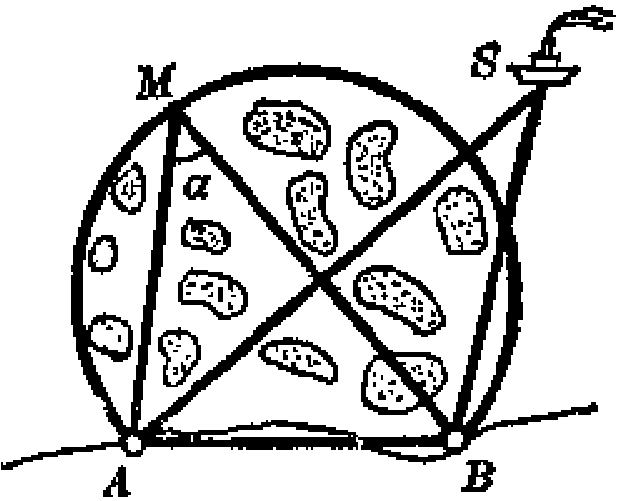
\includegraphics[width=5.5cm]{../pic/czjh2-ch7-26.png}
        \caption{}\label{fig:czjh2-7-26}
    \end{minipage}
\end{figure}


\liti 已知: 如图 \ref{fig:czjh2-7-25}, $P$ 是弓形 $AMB$ 内任意一点, $Q$ 是弓形外的任意一点,
并且和点 $P$ 在直线 $AB$ 同侧。弓形角等于 $\alpha$。

求证:(1) $\angle APB > \alpha$; (2)$\angle AQB < \alpha$。

\zhengming (1) 延长 $AP$ 交 $\yuanhu{AMB}$ 于点 $P'$。连结 $BP'$。

$\because$ \quad 点 $P'$ 在弓形弧上,

$\therefore$ \quad $\angle AP'B = \alpha$。

又 $\because$ \quad $\angle APB$ 是 $\triangle PP'B$ 的外角,

$\therefore$ \quad $\angle APB > \angle AP'B = \alpha$。

(2)设 $AQ$ 与 $\yuanhu{AMB}$ 交于点 $Q'$,连结 $BQ'$。

$\because$ \quad 点 $Q'$ 在弓形弧上,

$\therefore$ \quad $\angle AQ'B = \alpha$。

又 $\because$ \quad $\angle AQ'B$ 是 $\triangle BQ'Q$ 的外角。

$\therefore$ \quad $\angle AQB < \angle AQ'B = \alpha$。


例2 的结果,可以用来解决一些实际问题。
例如,临近暗礁的海岸上,可以建两个灯塔 $A$、$B$(图 \ref{fig:czjh2-7-26}),
使暗礁包围在以 $AB$ 为弦的弓形 $AMB$ 内。
那么只要航船 $S$ 能从所收到的信号中知道弓形角 $\alpha$ 的大小,
在航行中保持对两个灯塔的视角 $\angle ASB < \alpha$,航船就不会触礁。


\begin{lianxi}

\xiaoti{找出图中圆内接四边形对角线把 4 个内角分成的 8 个角中,哪些是相等的角。}

\begin{figure}[htbp]
    \centering
    \begin{minipage}[b]{4.5cm}
        \centering
        \begin{tikzpicture}
    \tkzDefPoints{0/0/O}
    \tkzDefPoint(160:1.5){A}
    \tkzDefPoint(220:1.5){B}
    \tkzDefPoint(320:1.5){C}
    \tkzDefPoint(70:1.5){D}

    \tkzDrawCircle[thick](O,A)
    \tkzDrawPolygon(A,B,C,D)
    \tkzDrawSegments(A,C  B,D)
    \tkzLabelPoints[left](A,B)
    \tkzLabelPoints[right](C)
    \tkzLabelPoints[above](D)
\end{tikzpicture}


        \caption*{(第 1 题)}
    \end{minipage}
    \qquad
    \begin{minipage}[b]{4.5cm}
        \centering
        \begin{tikzpicture} % 复杂
    % 利用:90度的圆周角所对的弦是直径
    \tkzDefPoints{0/0/O}
    \tkzDefPoint(60:1.5){B}
    \tkzDefPoint(190:2.0){D}
    \tkzDefTriangle[two angles=90 and 45](B,D)  \tkzGetPoint{E}
    \tkzInterLC[common=B](B,D)(O,B)  \tkzGetFirstPoint{A}
    \tkzInterLC[common=B](B,E)(O,B)  \tkzGetFirstPoint{C}

    \tkzDefLine[altitude](D,B,E)  \tkzGetPoint{H}
    \tkzDefPointOnLine[pos=0.3](B,H)  \tkzGetPoint{B'}
    \tkzDefPointBy[translation=from B to A](B')  \tkzGetPoint{d}
    \tkzDefPointOnLine[pos=0.6](B',d)  \tkzGetPoint{D'}
    \tkzDefTriangle[two angles=90 and 45](B',D')  \tkzGetPoint{E'}

    \tkzDrawCircle[thick](O,A)
    \tkzDrawPolygon[dashed](B,D,E)
    \tkzDrawPolygon[dashed](B',D',E')
    \tkzDrawSegments(A,C)
    \tkzLabelPoints[above left](A)
    \tkzLabelPoints[above](B)
    \tkzLabelPoints[above right](C)
\end{tikzpicture}


        \caption*{(第 2 题)}
    \end{minipage}
    \qquad
    \begin{minipage}[b]{4.5cm}
        \centering
        \begin{tikzpicture}
    \tkzDefPoints{0/0/O}
    \tkzDefPoint(180:1.5){A}
    \tkzDefPoint(80:1.5){B}
    \tkzDefMidPoint(A,O)  \tkzGetPoint{C}
    \tkzInterLC[common=A](A,B)(C,A)  \tkzGetFirstPoint{D}

    \tkzDrawCircle[thick](O,A)
    \tkzDrawCircle[thick](C,A)
    \tkzDrawSegments(A,O  A,B)
    \tkzDrawPoint(C)
    \tkzLabelPoints[left](A)
    \tkzLabelPoints[above](B,D)
    \tkzLabelPoints[below](C)
    \tkzLabelPoints[right](O)
\end{tikzpicture}


        \caption*{(第 3 题)}
    \end{minipage}
\end{figure}

\xiaoti{(口答)怎样运用三角板(或曲尺)作出圆形工件表面上的直径、定出圆心?说明理由。}

\xiaoti{$OA$ 是 $\yuan\,O$ 的半径,以 $OA$ 为直径的 $\yuan\,C$ 与 $\yuan\,O$ 的弦 $AB$
    相交于点 $D$。求证: $D$ 是 $AB$ 的中点。
}

\xiaoti{已知: $CD$ 是 $\triangle ABC$ 的中线, $AB = 2 CD$, $\angle B = 60^\circ$。
    求证: $\triangle ABC$ 外接圆的半径等于 $CB$。
}

\end{lianxi}
\end{enhancedline}

